\documentclass[aps,letterpaper,11pt]{revtex4}
\usepackage{graphicx} % For images
\usepackage{float}    % For tables and other floats
\usepackage{verbatim} % For comments and other
\usepackage{amssymb}  % For more math
\usepackage{fullpage} % Set margins and place page numbers at bottom center
\usepackage{listings} % For source code
\usepackage[usenames,dvipsnames]{color} % For colors and names
\usepackage[pdftex]{hyperref}           % For hyperlinks and indexing the PDF
\usepackage{pdfpages}
\usepackage{subfig}
\usepackage{listings}
\usepackage[usenames,dvipsnames,svgnames,table]{xcolor}
\usepackage{color}
\usepackage{textcomp}
\usepackage[utf8]{inputenc}
% Custom colors
\definecolor{deepblue}{rgb}{0,0,0.5}
\definecolor{deepred}{rgb}{0.6,0,0}
\definecolor{deepgreen}{rgb}{0,0.5,0}

 \lstset{
  tabsize=4,
  language=C++,
  captionpos=b,
  tabsize=3,
  numberstyle=\tiny,
  numbersep=5pt,
  breaklines=true,
  showstringspaces=false,
  basicstyle=\footnotesize,
%  identifierstyle=\color{magenta},
  keywordstyle=\color[rgb]{0,0,1},
  commentstyle=\color{deepgreen},
  stringstyle=\color{deepred}
  }
  
\hypersetup{ % play with the different link colors here
    colorlinks,
    citecolor=black,
    filecolor=black,
    linkcolor=black,
    urlcolor=blue % set to black to prevent printing blue links
}

\newcommand{\labno}{Personal Report N.1}
\newcommand{\labtitle}{Software Engineering Project}
\newcommand{\authorname}{Antoine Merlet}
\newcommand{\professor}{Dr. Yohan Fougerolle, Dr. Cansen Jiang, Dr. David Strubel}


\begin{document}  
\begin{titlepage}
\begin{center}
{\LARGE \textsc{\labno:} \\ \vspace{4pt}}
{\Large \textsc{\labtitle} \\ \vspace{4pt}} 
\rule[13pt]{\textwidth}{1pt} \\ \vspace{150pt}
{\large By: \authorname \\ \vspace{10pt}
Professor: \professor \\ \vspace{10pt}
\today}
\end{center}




\end{titlepage}% END TITLE PAGE %%%%%%%%%%%%%%%%%%%%%%%%%%%%%%%%%%
\newpage

This is my second report. In the past week, i focused on software design and code analysis


\section{Software design}

I tried to split as much as possible every aspect of the project so that, in the future, if our project has to be improved, it is possible to keep well designed and separated parts. In the previous codes, the GUI and the processing where not splitted, leading to strong difficulties regarding GUI modification. 
For the time being, I chose to focus on the design of the Input-Output. in fact, the function codes from previous students are good, they can only be improved regardign  their placement (too much in GUI files). Moreover, it is possible to have a good idea of the IO needs (and function declarations) without a deep study of it. I will discuss with Marcio on the viability of such a design according to his study of the IO sensors.

Regarding the GUI, I will wait for Mladen study before performing the design. Has he is in charge of this specific part, I will try by best to fulfill his needs when they will be stated.

On the matter of the storage, I think that none of the previous students managed it well, and I know that, from my knowledge, I will not be able to handle well either. While being use to proper database concept (Oracle, SQL), I am not sure on how to make a kind of database in C++ (meaningfull one). I will use next tutorial to ask my questions on this matter.

Finally, the Core package. I think it has to be the most raffined one. I will spend most of my time trying to make this part robust yet versatile. I started to put some function names I know we will for sure need. I will continue completing the design of this class when I will have more knowledge about PCL functions and datatypes, but also when Gulnur will have started to implement her mathematical tools and functions.

Below is shown the overall UML class diagram for our project.

\begin{figure}[H]
	\centering
	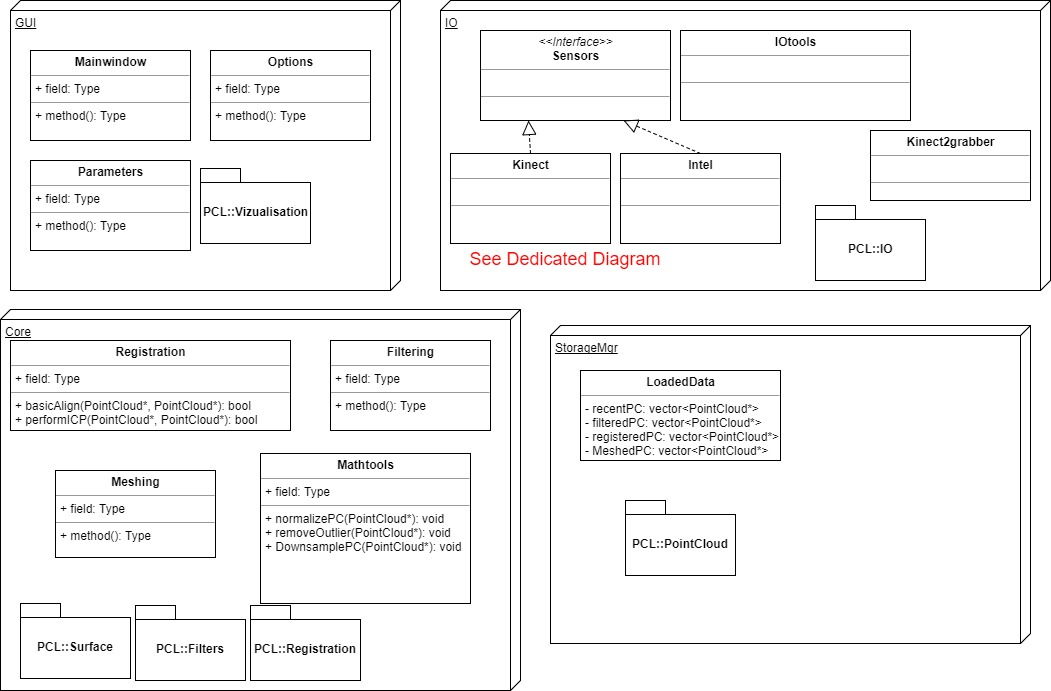
\includegraphics[width=15cm]{GeneralUML.jpg}
	\caption{General UML diagram: first draft}
	\label{fig: GeneralUML}    
\end{figure}

As I did no do proper software design in several years, my UML knowledge and my class splitting in general are a bit rusty. Therefore, Someone used to UML might find wrong use of several notations or concept. My go with this diagrams is to be understood by my teammates, by the future jury, and by myself. 
The presence of the PCL packages in each of my package (will certainly be namespace only) is here to show that the code is well splitted: we should not have to include PCL::IO in our GUI for example.

On the subject of IOs, following is shown the IO package UML diagram: 

\begin{figure}[H]
	\centering
	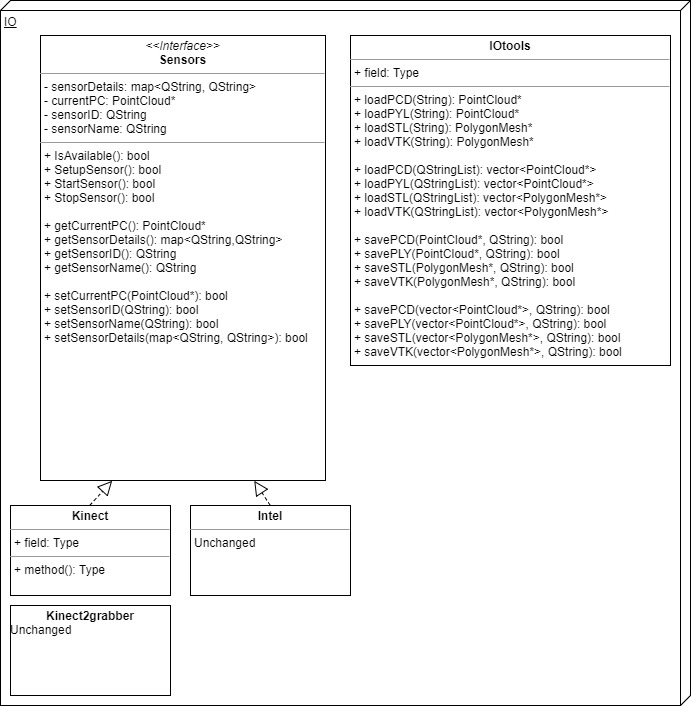
\includegraphics[width=15cm]{IODiagram.jpg}
	\caption{IO UML diagram: first version}
	\label{fig: IOUML}    
\end{figure}

This is the only precised package yet, and it still can be improved


\section{Future work}

I will continue, every time I think it is necessary, to change the ULM class diagrams. Normally, this UML should be fully finished before starting coding, but we have limited time and knowledge. Our project will not be perfect. Lets just make it as good as possible.
The coming week, I will create the project structure and already designed function, manage the CMake/QMake files, and upload the code.

\end{document} % DONE WITH DOCUMENT!

